\documentclass[18 pt]{beamer}
\usetheme{Madrid}
% \usefonttheme{professionalfonts}
\usefonttheme{structurebold}
\usecolortheme{rose}
\usepackage{tcolorbox}
\setbeamerfont{title}{size=\LARGE, series=\bfseries}
\title{Synthesis on Atom Computation}


\usepackage{amsmath}
\usepackage{amssymb}
\usepackage{listings}
\usepackage{booktabs}
\usepackage{multirow}
\usepackage{multirow}
\usepackage{lmodern}
\usepackage{xcolor}
\usepackage{float}
\lstset{
  language=Python,  %代码语言使用的是matlab
  % frame=shadowbox, %把代码用带有阴影的框圈起来
  rulesepcolor=\color{red!20!green!20!blue!20},%代码块边框为淡青色
  keywordstyle=\color{blue!90}\bfseries, %代码关键字的颜色为蓝色,粗体
  commentstyle=\color{red!10!green!70}\textit,    % 设置代码注释的颜色
  basicstyle=\footnotesize,
  showstringspaces=true,%不显示代码字符串中间的空格标记
  % numbers=left, % 显示行号
  % numberstyle=8pt,    % 行号字体
  % numberstyle=\color{green},
  stringstyle=\rmfamily\slshape\color[RGB]{128,0,0}, % 代码字符串的特殊格式
  breaklines=true, %对过长的代码自动换行
  extendedchars=false,  %解决代码跨页时,章节标题,页眉等汉字不显示的问题
  escapeinside=``,%代码中出现中文必须加上,否则报错
  texcl=true}

\lstset{breaklines}%自动将长的代码行换行排版

\lstset{extendedchars=false}%解决代码跨页时,章节标题,页眉等汉字不显示的问题

\usepackage{textcomp}
% \usepackage[margin=1in]{geometry}
\usepackage{pythonhighlight}
% \usepackage{minted}
\usepackage[backend=bibtex]{biblatex}
%\usepackage[style=authortitle,backend=biber]{biblatex}
\addbibresource{ResearchRabbit_Export_2022_10_20.bib}

\usepackage{algorithm}
\usepackage{algorithmic}
\renewcommand{\algorithmicrequire}{\textbf{Input:}}
\renewcommand{\algorithmicensure}{\textbf{Output:}}


\setbeamertemplate{footline}[frame number]
\begin{document}
\begin{frame}[plain]
    \titlepage
\end{frame}
\section{Compilation for Dynamically Field-Programmable Qubit Arrays with Efficient and Provably Near-Optimal Scheduling}
\begin{frame}
    \frametitle{Related Works}
    \begin{itemize}
        \item \textbf{\textit{Compiling Quantum Circuits for Dynamically Field-Programmable Neutral Atoms Array Processors}}: Utilizes Z3 MST, but lacks scalability and fidelity considerations.
        \item \textbf{\textit{FPQA-C: A Compilation Framework for Field Programmable Qubit Array}}: Employs a rule-based algorithm, offering good scalability, but does not achieve the optimal count of 2Q gates.
    \end{itemize}
    \begin{figure}
        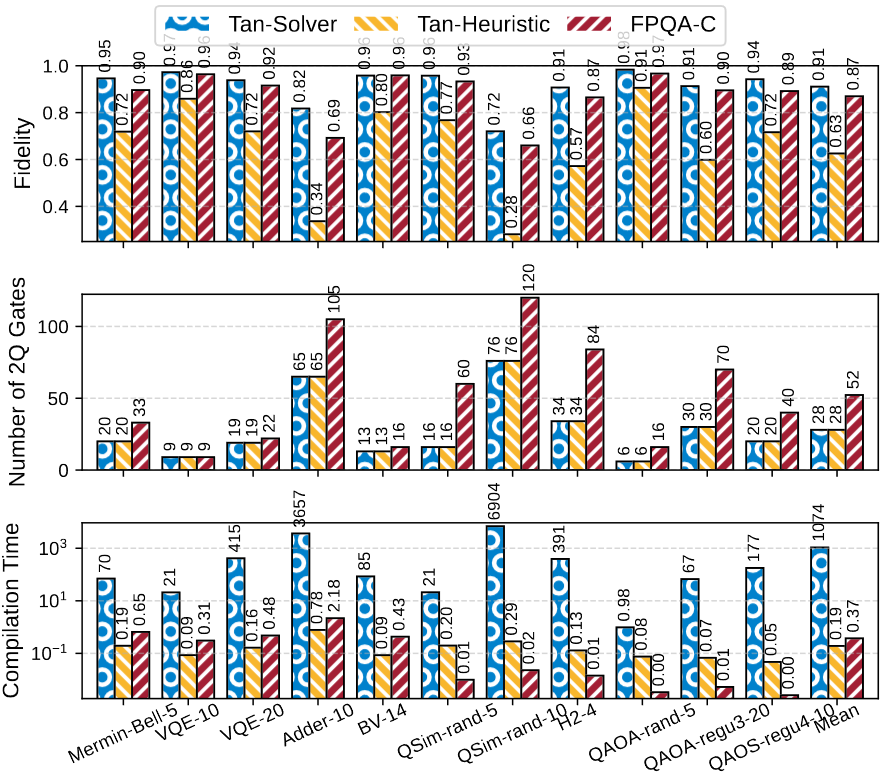
\includegraphics[height=5cm]{back.png}
    \end{figure}
\end{frame}

\begin{frame}
    \frametitle{Overview}
    \begin{itemize}
        \item Background: Quantum computing with neutral atoms has advanced rapidly.
        \item Fidelity: \(f=\left(f_{1}\right)^{g_{1}} \cdot \overbrace{\left(f_{2}\right)^{g_{2}} \cdot\left(f_{\text {exc }}\right)^{|Q| S-2 g_{2}}}^{\text {two-qubit gate }} \cdot \overbrace{\left(f_{\text {trans }}\right)^{N_{\text {trans }}}}^{\text {atom transfer }}\cdot \overbrace{\prod_{q\in Q} (1-T_q/T_2)}^{decoherence}\).
        \item Significant scalability: experiments with up to 6,100 qubits.
        % \item Challenges in fully leveraging hardware flexibility while respecting constraints.
        \item The compilation process is broken down into three tasks: scheduling, placement, and routing.
    \end{itemize}
    \begin{table}[h!]
        \centering
        \tiny
        \begin{tabular}{|c|c|c|c|c|c|c|}
        \hline
        \textbf{Qubit Num} & \textbf{Gate Num} & \textbf{Scheduling} & \textbf{Placement} & \textbf{Routing} & \textbf{Codegen} & \textbf{Total} \\
        \hline
        30 & 45 & 0.0008 & 137.32 & 0.0057 & 0.0184 & 137.35 \\
        \hline
        60 & 60 & 0.0017 & 141.23 & 0.0124 & 0.0379 & 141.28 \\
        \hline
        90 & 135 & 0.0023 & 144.43 & 0.0304 & 0.0630 & 144.52 \\
        \hline
        \end{tabular}
        \caption{Timing Results for Different Qubit and Gate Numbers}
        \label{table:timing_results}
    \end{table}
\end{frame}

\begin{frame}
    \frametitle{Scheduling}
    \begin{itemize}
        \item Scheduling is crucial for determining the sequence of operations. Graph edge coloring is used to model the scheduling problem.
        \item Each edge represents a two-qubit gate.
        \item Colors represent different stages.
        % \item Ensures near-optimal stage count for two-qubit gates.
        % \item Proven to be at most one stage more than the optimal solution.
        % \item This reduces the fidelity bottleneck in this platform.
        \item The goal is to minimize the number of stages while ensuring no two adjacent edges share the same color.
    \end{itemize}
    \begin{figure}
        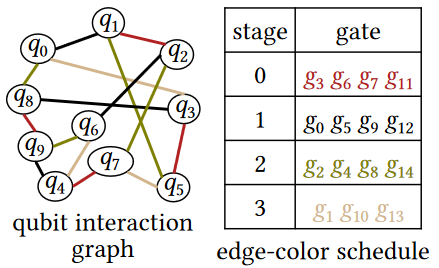
\includegraphics[height=4.5cm]{color.png}
    \end{figure}
    
\end{frame}

\begin{frame}
    \frametitle{Scheduling: Graph Edge Coloring}
    \begin{theorem}
        \textbf{Vizing's Theorem:} For any simple graph \( G \) with maximum degree \( \Delta \), the chromatic index \(\chi'(G)\) satisfies:
\[
\Delta \leq \chi'(G) \leq \Delta + 1
\]
where \(\chi'(G)\) is the minimum number of colors needed to color the edges of \( G \).

    \end{theorem}
    \begin{itemize}
        \item There exists an algorithm with runtime \( O(|V| \cdot |E|) \) that provides an edge coloring \(\phi: E \to \{0, 1, 2, \dots, \Delta(G)\}\).
        \item The maximum gate count is \( \binom{n}{2} \). Thus, the time complexity of scheduling is \( O(n^3) \).
    \end{itemize}    
\end{frame}

\begin{frame}
    \frametitle{Placement}
    \begin{itemize}
        \item Placement refers to assigning qubits to physical locations.
        \item Optimal placement minimizes the distance between interacting qubits.
        \item This reduces the need for long-distance routing, which can lower fidelity.
    \end{itemize}
    \begin{block}{Formula}
        \[
        \sum_{g(q,q') \in G} w_g \cdot \text{dist}(m(q), m(q'))
        \]
        
        where \( w_g \) is the weight for gate \( g \), \( m \) is the placement function from qubits to interaction sites, and \(\text{dist}\) is the \textbf{Euclidean distance}.
    \end{block}
\end{frame}

\begin{frame}
    \frametitle{Placement Strategies}
    \begin{itemize}
        \item Use of simulated annealing algorithms to find near-optimal solutions with a constant runtime.
        \item Balancing between computational efficiency and placement quality.
        \[
x \in \left[0, \max\left(\lfloor \sqrt{n} \rfloor + 4, x_{\max}\right)\right],
y \in \left[0, \max\left(\lfloor \sqrt{n} \rfloor + 4, y_{\max}\right)\right]
\]
        % \item Consideration of hardware constraints and qubit connectivity.
    \end{itemize}
    \begin{block}{Formula}
        \begin{align*}
            w_g & = \begin{cases}
            1, &\text{static placement}
             \\ 
            \max\left(0.1,1-0.1s_g\right), &\text{dynamic placement}
            \end{cases}
        \end{align*}
    \end{block}
\end{frame}
\begin{frame}
    \frametitle{Placement example}
    \begin{figure}
        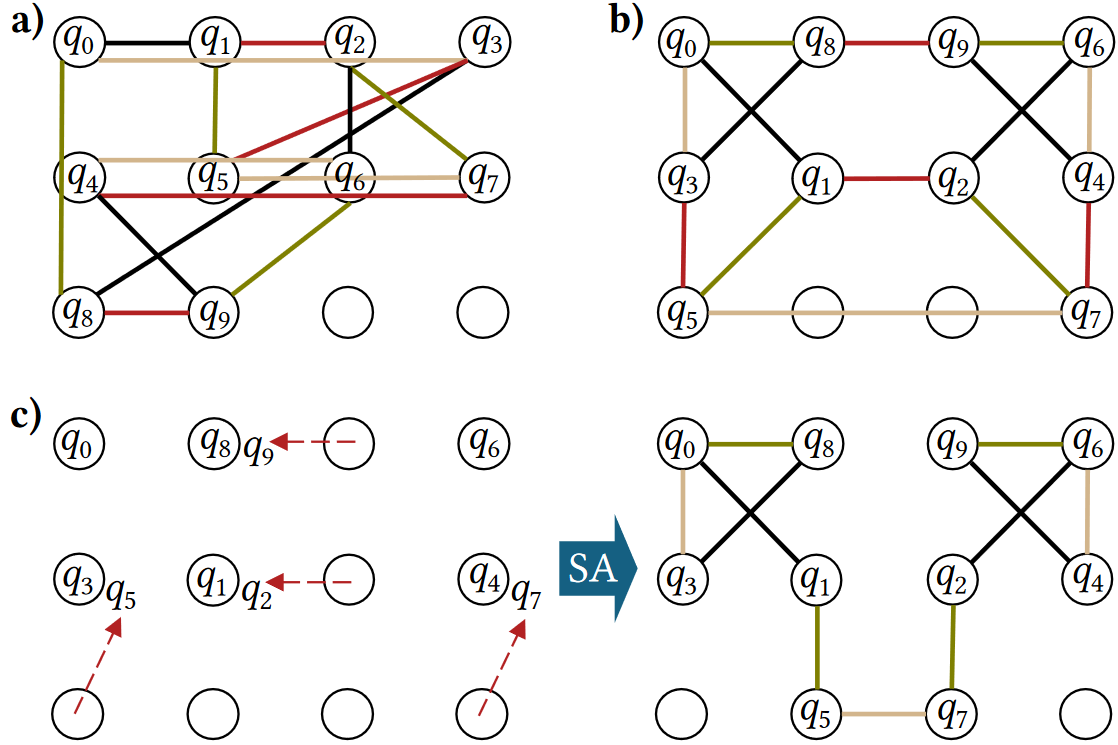
\includegraphics[height = 8cm]{placement.png}
    \end{figure}
\end{frame}

\begin{frame}
    \frametitle{Routing}
    \begin{itemize}
        \item Routing involves determining paths for qubits to move during computation. Ensuring minimal delay and avoiding congestion are key goals.
        \item A conflict graph represents the conflicts during the routing process.
        \item Nodes represent qubits movements, and edges represent conflicts.
        \item The problem is The Maximum Independent Set (MIS) problem, where one seeks to find the largest set of vertices in a graph such that no two vertices in the set are adjacent.
    \end{itemize}
    \begin{figure}
        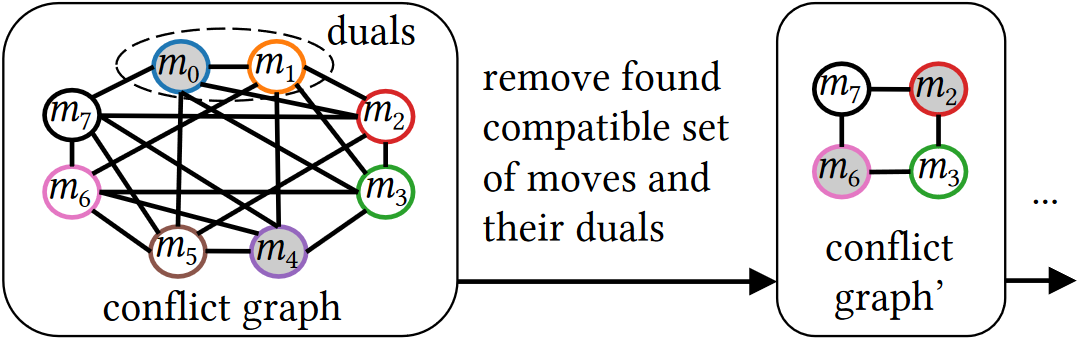
\includegraphics[height=3.5cm]{conflict.png}
    \end{figure}
\end{frame}

\begin{frame}
    \frametitle{Greedy Algorithm for Bounded Degree Graphs}
    \begin{enumerate}
        \item putting all vertices in a list (sorted by distance).
        \item adding the first vertex to the IS.
        \item removing all its neighbors from the list, and continuing 2-3.
    \end{enumerate}
   \begin{Theorem}
    In bounded degree graphs, there are effective approximation algorithms with constant ratios. For example, a greedy algorithm that forms a maximal independent set by repeatedly choosing the vertex with the minimum degree and removing its neighbors achieves an approximation ratio of $(\Delta + 2)/3$ for graphs with maximum degree $\Delta$. Approximation hardness bounds for these cases were shown by Berman and Karpinski (1999).
   \end{Theorem}
\end{frame}
\begin{frame}
    \frametitle{Routing Complexity}
    For the number of qubits $n$, the maximum number of gates is $n/2$, so the number of vertices is at most $n$ ($|V| \leq n$):
    \begin{itemize}
        \item Checking conflicts for all pairs of vertices requires $O(|V|^2)$ time.
        \item Sorting the vertices requires $O(|V|\log |V|)$ time.
        \item The greedy algorithm requires $O(|V|^2)$ time. In the worst case, the greedy algorithm needs to be run $O(|V|)$ times.
        \item \textbf{In total, there can be $O(n)$ Rydberg stages, resulting in a routing time of $O(n^4)$.}
    \end{itemize}
    \vspace{10pt}
    Only construct a graph on the first $K$ vertices in the lists ($|V| = K$):
    \begin{itemize}
        \item \textbf{The windowed routing takse $O(n^2\log n + n^2K^2)$.}
    \end{itemize}
\end{frame}

\begin{frame}
    \frametitle{Results and Comparison}
    \begin{itemize}
        \item The compiler, Enola, shows significant improvements in performance.
        \item Achieves 3.7X stage reduction compared to existing works.
        \item Demonstrates 5.9X improvement in fidelity on benchmark sets.
        \item Highly scalable, capable of compiling circuits with up to 10,000 qubits within 30 minutes.
        \item Outperforms the current state of the art, OLSQ-DPQA.
    \end{itemize}
\end{frame}

\begin{frame}
    \frametitle{Conclusion}
    \begin{itemize}
        \item The compilation process for dynamically field-programmable qubit arrays involves scheduling, placement, and routing.
        \item The method provide near-optimal solutions for scheduling ($S_{opt} +1$) and efficient strategies for placement and routing.
        \item Enola compiler achieves significant improvements in stage reduction and fidelity.
        \item Future work includes further optimization and exploring additional constraints.
        \item Open source availability: \url{https://github.com/UCLA-VAST/Enola}
    \end{itemize}
\end{frame}

\section{Computational capabilities and compiler development for neutral atom quantum processors—connecting tool developers and hardware experts}
\begin{frame}
    \frametitle{<title>}

    

\end{frame}
\end{document}
